% documentclass: article used for scientific journals, short reports, program documentation, etc
% options: fontsize 11, generate document for double sided printing, a4-paper
\documentclass[10pt, twoside, a4paper]{article}

% package for changing page layout
\usepackage{geometry}
\geometry{a4paper, lmargin=40mm, rmargin=45mm, tmargin=40mm, bmargin=45mm}
% set indentation
\setlength{\parindent}{1em}
% set factor for line spacing
% \linespread{1.0}\selectfont
% set (dynamic) additional line spacing
% \setlength{\parskip}{1ex plus 0.5ex minus 0.3ex}

% rigorous formatting (not too much hyphens)
% \fussy
% \sloppy

% package for changing page layout (used to indent whole paragraphs with adjustwidth)
\usepackage{changepage}

% input encoding for special characters (e.g. ä,ü,ö,ß), only for non english text
% options: utf8 as encoding standard, latin1
\usepackage[utf8]{inputenc}
% package for font encoding
\usepackage[T1]{fontenc}
% package for changing used language (especially for more than one language)
% options: ngerman (new spelling) or default: english
\usepackage[ngerman]{babel}
% package for times font
% \usepackage{times}
% package for latin modern fonts
\usepackage{lmodern}

% package for math symbols, functions and environments from ams(american mathematical society)
\usepackage{amsmath}
\usepackage{mathtools}
% package for extended symbols from ams
\usepackage{amssymb}
% package for math black board symbols (e.g. R,Q,Z,...)
\usepackage{bbm}
% package used for calligraphic math symbols
\usepackage{mathrsfs}
% package for extended symbols from stmaryrd(st mary road)
\usepackage{stmaryrd}
% package for more math blackboard symbols
\usepackage{dsfont}

% pack­age im­ple­ments scal­ing of the math ex­ten­sion font cmex; used for scaling math signs
\usepackage{exscale}

% package for including extern graphics plus scaling and rotating
\usepackage{graphicx}
%package for positioning figures
\usepackage{float}
% package for changing color of font and paper
% options: using names of default colors (e.g red, black)
% \usepackage[usenames]{color}
\usepackage[dvipsnames]{xcolor}
\definecolor{shadecolor}{gray}{0.9}
% package for customising captions
\usepackage[footnotesize, hang]{caption}
% package for customising enumerations (e.g. axioms)
\usepackage{enumitem}
% calc package reimplements \setcounter, \addtocounter, \setlength and \addtolength: commands now accept an infix notation expression
\usepackage{calc}
% package for creating framed, shaded, or differently highlighted regions that can break across pages; environments: framed, oframed, shaded, shaded*, snugshade, snugshade*, leftbar, titled-frame
\usepackage{framed}
% package for creating custom "list of"
% options: titles: do not intefere with standard headings for "list of"
\usepackage[titles]{tocloft}
% change enumeration style of equations
% \renewcommand\theequation{\thesection.\arabic{equation}}

% init list of math for definitions and theorems
\newcommand{\listofmathcall}{Verzeichnis der Definitionen und Sätze}
\newlistof{math}{mathlist}{\listofmathcall}
% add parentheses around argument
\newcommand{\parent}[1]{ \ifx&#1&\else (#1) \fi }
% unnumerated mathematical definition environment definiton
\newenvironment{mathdef*}[2]{
	\begin{tcolorbox}[colback=white, boxrule=0.5pt, enhanced, colframe=black]
	\noindent
	{ \fontfamily{ppl}\selectfont \textbf{\textsc{#1:}} } ~ #2 
	\par \hfill\\ 
	\fontfamily{lmr}\selectfont \itshape
}{
	\end{tcolorbox}
}
% definitions for numerated mathematical definition environment
\newcounter{mathdefc}[section]
\newcommand*{\mathdefnum}{\thesection.\arabic{mathdefc}}
\renewcommand{\themathdefc}{\mathdefnum}
\newenvironment{mathdef}[2]{
	\refstepcounter{mathdefc}
	\addcontentsline{mathlist}{figure}{\protect{\numberline{\mathdefnum}#1 ~ #2}}
	\begin{mathdef*}{#1 \mathdefnum}{#2}
}{
	\end{mathdef*}
}
% standard mathdef calls
\newcommand{\definitioncall}{Definition}
\newenvironment{definition*}[1][]{ \begin{mathdef*}{\definitioncall}{\parent{#1}} }{ \end{mathdef*} }
\newenvironment{definition}[1][]{ \begin{mathdef}{\definitioncall}{\parent{#1}} }{ \end{mathdef} }
% unnumerated theorem environment definition
\newenvironment{maththeorem*}[2]{
	\begin{leftbar}%[boxrule=0pt, leftrule=3pt, arc=0pt, colback=white, colframe=black, enhanced jigsaw]
	\noindent
	{ \fontfamily{ppl}\selectfont \textbf{\textsc{#1:}} } ~ #2
	\par \hfill\\ 
	\fontfamily{lmr} \fontshape{it} \selectfont
}{ 
	\end{leftbar}
}
% definitions for numerated theorem environment
\newcounter{maththeoremc}[section]
\newcommand*\maththeoremnum{\thesection.\arabic{maththeoremc}}
\renewcommand{\themaththeoremc}{\maththeoremnum}
\newenvironment{maththeorem}[2]{
	\refstepcounter{maththeoremc}
	\addcontentsline{mathlist}{figure}{\protect{\qquad\numberline{\maththeoremnum}#1 ~ #2}}
	\begin{maththeorem*}{#1 \maththeoremnum}{#2}
}{
	\end{maththeorem*}
}
% standard maththeorem calls
\newcommand{\theoremcall}{Theorem}
\newenvironment{theorem*}[1][]{ \begin{maththeorem*}{\theoremcall}{\parent{#1}} }{ \end{maththeorem*} }
\newenvironment{theorem}[1][]{ \begin{maththeorem}{\theoremcall}{\parent{#1}} }{ \end{maththeorem} }
\newcommand{\lemmacall}{Lemma}
\newenvironment{lemma*}[1][]{ \begin{maththeorem*}{\lemmacall}{\parent{#1}} }{ \end{maththeorem*} }
\newenvironment{lemma}[1][]{ \begin{maththeorem}{\lemmacall}{\parent{#1}} }{ \end{maththeorem} }
\newcommand{\propositioncall}{Proposition}
\newenvironment{proposition*}[1][]{ \begin{maththeorem*}{\propositioncall}{\parent{#1}} }{ \end{maththeorem*} }
\newenvironment{proposition}[1][]{ \begin{maththeorem}{\propositioncall}{\parent{#1}} }{ \end{maththeorem} }
\newcommand{\corollarycall}{Korollar}
\newenvironment{corollary*}[1][]{ \begin{maththeorem*}{\corollarycall}{\parent{#1}} }{ \end{maththeorem*} }
\newenvironment{corollary}[1][]{ \begin{maththeorem}{\corollarycall}{\parent{#1}} }{ \end{maththeorem} }
% q.e.d. definition
\newcommand{\qed}{ \par \hfill \fontfamily{lmr} \fontshape{it} \selectfont \mbox{q.e.d.} \\}
\newcommand{\qedbox}{ \par \hfill $\Box$ \\ }
% proof environment definition for theorems
\newenvironment{mathproof}[1]{
	\par\hfill\\
	\noindent
	{ \fontfamily{lmr}\selectfont \small \textsc{#1:}}
	\normalfont
	\small
	\begin{adjustwidth}{1em}{}
	\medskip
}{ 
	\end{adjustwidth} 
	% \qed
	\qedbox
}
% standard mathproof calls
\newcommand{\proofcall}{Beweis}
\newenvironment{proof}{ \begin{mathproof}{\proofcall} }{ \end{mathproof} }
\newcommand{\proofideacall}{Beweisidee}
\newenvironment{proofidea}{ \begin{mathproof}{\proofideacall} }{ \end{mathproof} }

% new displaymath command, so that equations will not be stretched
\newcommand{\D}[1]{\mbox{$ #1 $}}
% make unnumerated equation
\newcommand{\E}[1]{\[ #1 \]}
% command for curly brackets
\newcommand{\curlb}[1]{\left\{ #1 \right\}}
% command for box brackets
\newcommand{\boxb}[1]{\left[ #1 \right]}
% command for parentheses/curved brackets
\newcommand{\curvb}[1]{\left( #1 \right)}
% command for angle brackets
\newcommand{\angleb}[1]{\left\langle #1 \right\rangle}
% command for floor brackets
\newcommand{\floorb}[1]{\left\lfloor #1 \right\rfloor}
% command for ceil brackets
\newcommand{\ceilb}[1]{\left\lceil #1 \right\rceil}
% command for creating sets
\newcommand{\set}[2]{ \left\{ #1 \enspace \middle\vert \enspace #2 \right\} }
% command for absolute value
\newcommand{\abs}[1]{\left\vert #1 \right\vert}
\newcommand{\norm}[1]{\left\| #1 \right\|}
% commands for writing limits
\newcommand{\limit}[3]{\, \longrightarrow \, #1, \ #2 \longrightarrow #3}
\newcommand{\Limit}[2]{\lim_{#1 \rightarrow #2}}
% command for differential
\newcommand{\diff}{\mathrm{d}}
\newcommand{\Diff}{\mathrm{D}}
% command for derivative
\newcommand{\Deriv}[3][]{\Diff_{#2}^{#1}#3}
\newcommand{\deriv}[3][]{\dfrac{\diff^{#1}#2(#3)}{\diff #3^{#1}}}
% command for integral
\newcommand{\integral}[4]{\int_{#1}^{#2} #3\ \diff #4}
\newcommand{\Integral}[4]{\int\limits_{#1}^{#2} #3\ \diff #4}
\newcommand{\iintegral}[2]{\int #1\ \diff #2} % indefinite integral
% mathematical definitions (standard sets)
\newcommand{\SR}{\mathds{R}} % real numbers
\newcommand{\SC}{\mathds{C}} % complex numbers
\newcommand{\SN}{\mathds{N}} % natural numbers
\newcommand{\SZ}{\mathds{Z}} % integral numbers
\newcommand{\SQ}{\mathds{Q}} % rational numbers
\newcommand{\SP}{\mathcal{P}} % power set
\newcommand{\SFP}{\mathds{P}} % polynom functions
\newcommand{\SFC}{\mathrm{C}} % complex valued functions (continous or differentiable)
\newcommand{\SFL}{\mathcal{L}} % space of integrable functions
\newcommand{\SFLL}{\mathrm{L}} % space of integrable function classes
\newcommand{\SH}{\mathcal{H}} % hilbert space
% mathematical standard functions
\DeclareMathOperator{\real}{Re} % real part
\DeclareMathOperator{\imag}{Im} % imaginary part
\newcommand{\FF}{\mathcal{F}} % fourier transform
\newcommand{\FE}{\mathbb{E}} % expectation
\DeclareMathOperator{\var}{var} % variance
\newcommand{\FN}{\mathcal{N}} % normal distribution

% command for physical units
\newcommand{\unit}[1]{\, \mathrm{#1}}


% package for init listings(non-formatted  text) e.g. different source codes
\usepackage{listings}


% definitions for listing colors
\definecolor{codeDarkGray}{gray}{0.2}
\definecolor{codeGray}{gray}{0.4}
\definecolor{codeLightGray}{rgb}{0.94,0.94,0.91}
\definecolor{codeBorder}{rgb}{0.34,0.24,0.21}
% predefinitions for listings
\newcommand{\listingcall}{Listing}
\newlength{\listingframemargin}
\setlength{\listingframemargin}{1em}
\newlength{\listingmargin}
\setlength{\listingmargin}{0.08\textwidth}
% \newlength{\listingwidth}
% \setlength{\listingwidth}{ ( \textwidth - \listingmargin * \real{2} + \listingframemargin * \real{2} ) }
% definitions for list of listings
\newcommand{\listoflistingscall}{\listingcall -Verzeichnis}
\newlistof{listings}{listinglist}{\listoflistingscall}
% style definition for standard code listings
\lstdefinestyle{std}{
	belowcaptionskip=0.5\baselineskip,
	breaklines=true,
	frameround=tttt,
	% frame=false,
	xleftmargin=0em,
	xrightmargin=0em,
	showstringspaces=false,
	showtabs=false,
	% tab=\smash{\rule[-.2\baselineskip]{.4pt}{\baselineskip}\kern.5em},
	basicstyle= \fontfamily{pcr}\selectfont\footnotesize\bfseries,
	keywordstyle= \bfseries\color{MidnightBlue}, %\color{codeDarkGray},
	commentstyle= \itshape\color{codeGray},
	identifierstyle=\color{codeDarkGray},
	stringstyle=\color{BurntOrange}, %\color{codeDarkGray},
	numberstyle=\tiny\ttfamily,
	% numbers=left,
	numbersep = 1em,
	% stepnumber = 1,
	% captionpos=t,
	tabsize=4,
	% backgroundcolor=\color{codebLightGray},
	rulecolor=\color{codeBorder},
	framexleftmargin=\listingframemargin,
	framexrightmargin=\listingframemargin
}
% definition for unnumerated listing
\newcommand{\inputlistingn}[3][]{
	\begin{center}
		\begin{adjustwidth}{\listingmargin}{\listingmargin}
			\centerline{ {\fontfamily{lmr}\selectfont \footnotesize \listingcall:}\quad {\footnotesize #2} }
			\lstinputlisting[style=std, #1]{#3}
		\end{adjustwidth}
	\end{center}
}
% definition for numerated listing
\newcounter{listingc}[section]
\newcommand*\listingnum{\thesection.\arabic{listingc}}
\renewcommand{\thelistingc}{\listingnum}
\newcommand{\inputlisting}[3][]{
	\refstepcounter{listingc}
	\addcontentsline{listinglist}{figure}{\protect{\numberline{\listingnum:} #2 } }
	% \inputlistingn[#1]{#2}{#3}
	\begin{center}
		\begin{adjustwidth}{\listingmargin}{\listingmargin}
			\centerline{ {\fontfamily{lmr}\selectfont \footnotesize \listingcall~\listingnum:}\quad {\footnotesize #2} }
			\lstinputlisting[style=std, #1]{#3}
		\end{adjustwidth}
	\end{center}
}


% package for including csv-tables from file
% \usepackage{csvsimple}
% package for creating, loading and manipulating databases
\usepackage{datatool}

% package for converting eps-files to pdf-files and then include them
\usepackage{epstopdf}
% use another program (ps2pdf) for converting
% !!! important: set shell_escape=1 in /etc/texmf/texmf.cnf (Linux/Ubuntu 12.04) for allowing to use other programs
% !!!			or use the command line with -shell-escape
% \epstopdfsetup{outdir=./}
% \epstopdfDeclareGraphicsRule{.eps}{pdf}{.pdf}{
% ps2pdf -dEPSCrop #1 \OutputFile
% }


% package for reference to last page (output number of last page)
\usepackage{lastpage}
% package for using header and footer
% options: automate terms of right and left marks
\usepackage[automark]{scrpage2}
% \setlength{\headheight}{4\baselineskip}
% set style for footer and header
\pagestyle{scrheadings}
% \pagestyle{headings}
% clear pagestyle for redefining
\clearscrheadfoot
% set header and footer: use <xx>head/foot[]{Text} (i...inner, o...outer, c...center, o...odd, e...even, l...left, r...right)

% use that for mark to last page: \pageref{LastPage}
% set header separation line
\setheadsepline[\textwidth]{0.5pt}
% set foot separation line
\setfootsepline[\textwidth]{0.5pt}



\usepackage{tcolorbox}
% \usepackage{tikz}
% \tcbuselibrary{listings}
\tcbuselibrary{many}
\tcbset{fonttitle=\footnotesize}

\usepackage{array}

\allowdisplaybreaks

% \usepackage{epic, eepic}
\usepackage{epic}

\usepackage{natbib}
\bibliographystyle{plain}
\usepackage{url}


\ihead[]{Handout: \\ Fast Fourier Transform}
\ohead[]{Markus Pawellek \\ markuspawellek@gmail.com}
\cfoot[]{\newline\newline\newline\pagemark}

\title{Handout - Fast Fourier Transform}
\author{Markus Pawellek}
\date{03.Februar 2016}

\begin{document}
	
	\maketitle
	% \tableofcontents
	% \newpage
	\thispagestyle{empty}
	% \null
	% \newpage
	% \pagenumbering{arabic}

	\section{Mathematische Grundlagen} % (fold)
	\label{sec:mathematische_grundlagen}

		% Alle Betrachtungen beziehen sich im Allgemeinen auf periodische Funktionen.
		
		% \begin{itemize}
		% 	\item $T\in(0,\infty)$
		% 	% \item $f:\SR\longrightarrow\SC$ ist $T$-periodisch
		% 	\item $n\in\SN$
		% 	\item $\mathrm{N}_{n} := \curlb{0,\ldots,n-1}$
		% \end{itemize}

		\begin{definition*}[periodische Funktionen]
			Sei $T\in(0,\infty)$.
			Eine Abbildung $f:\SR\longrightarrow\SC$ heißt dann $T$-periodisch, wenn für alle $x\in\SR$ gilt
			$$ f(x) = f(x+T) $$
			In diesem Falle nennt man $T$ auch die Periode von $f$ und $1/T$ auch die Frequenz von $f$.
		\end{definition*}
		Für die folgenden Aussagen soll $T\in(0,\infty)$ immer die Periode einer Funktion beschreiben.

		\subsection{Fouriertransformation periodischer Funktionen} % (fold)
		\label{sub:fouriertransformation_periodischer_funktionen}
		
			\begin{definition*}[Fouriertransformation]
				% Sei $T\in(0,\infty)$.
				Für eine $T$-periodische Funktion $f:\SR\longrightarrow\SC$, welche stückweise stetig differenzierbar ist, kann man die Fouriertransformation $\FF$ und ihre Inverse definieren durch
				\begin{alignat*}{4}
					&\forall k\in\SZ:\quad &\FF f(k) &:= &&\ \frac{1}{T}\integral{0}{T}{ f(x)\exp\curvb{ -\frac{2\pi i}{T}kx } }{x} \\
					&\forall x\in\SR:\quad &f(x) &:= &&\ \sum_{k\in\SZ}\FF f(k)\exp\curvb{ \frac{2\pi i}{T}kx }
				\end{alignat*}
			\end{definition*}

			Die Fouriertransformation spaltet damit gerade eine periodische Funktion $f$ in sogenannte Frequenzanteile auf.
			Ein solcher Frequenzanteil beschreibt dann, zu welchem Anteil die harmonische Schwingung $\exp(i\omega\cdot)$ der angegebenen Frequenz $\omega/2\pi$ in der Funktion vorkommt.
			
			Diese Transformation lässt sich auch noch für andere Funktionen einführen.
			Für eine genauere Betrachtung der dahinter stehenden Mathematik sei hier auf die Quellen \cite{stein-fa} und \cite{elstrodt-mit} verwiesen.

		% subsection fouriertransformation_periodischer_funktionen (end)

		\subsection{Diskrete Fouriertransformation} % (fold)
		\label{sub:diskrete_fouriertransformation}

			Bekannterweise lassen sich in einem Computer Reihen fast immer nur approximieren, da die Addition unendlich vieler Glieder ungleich Null in endlicher Zeit auf endlichem Speicherplatz nicht durchführbar ist.
			Aus diesem Grund führt man die diskrete Fouriertransformation ein, welche in gewisser Weise eine Näherung der Vorhergehenden ist.

			Es sei nun immer $n\in\SN$ und $\mathrm{N}_{n} := \curlb{0,\ldots,n-1}$.
			Misst man in der Realität nun einen Zusammenhang $f$, so lässt sich diese nur näherungsweise durch Stützstellen $x_0,\ldots,x_{n-1} \in [0,T)$ mit den zugehörigen Funktionswerten $f(x_0),\ldots,f(x_{n-1})$ beschreiben.
			In diesen und folgenden Betrachtungen sollen alle Stützstellen als äquidistant angenommen werden.
			Die Funktion wurde diskretisiert.
			Man definiert nun
			\[ g:\mathrm{N}_n\longrightarrow\SC,\qquad g(k):=f(x_k) \]
			$g$ stellt damit ein Element des $\SC^n$ dar.
			Es lässt sich also jede diskretisierte Funktion als komplexer $n$-dimensionaler Vektor darstellen.
			Weiterhin sei für alle $x,y\in\SC^n$
			\[ \angleb{\cdot,\cdot}:\SC^n\times\SC^n\longrightarrow\SC,\qquad \angleb{x,y}:=\frac{1}{n}\sum_{j=0}^{n-1} \overline{x(i)}y(i) \]
			Die Abbildung $\angleb{\cdot,\cdot}$ definiert gerade das Standardskalarprodukt des $\SC^n$.
			Das Tupel $\curvb{ \SC^n, \angleb{\cdot,\cdot} }$ muss dann ein Hilbertraum sein.
			Dies ermöglicht es eine Orthonormalbasis zu finden.
			\begin{proposition*}[Orthonormalbasis]
				Die folgende Menge $D$ bildet eine Orthonormalbasis des $\curvb{ \SC^n, \angleb{\cdot,\cdot} }$.
				\[ D := \set{\omega_k:\mathrm{N}_n\longrightarrow\SC}{ k\in\mathrm{N}_n,\ \forall x\in\mathrm{N}_n:\ \omega_k(x) = \exp\curvb{\frac{2\pi i}{n}kx} } \]

				% \begin{proof}
				% 	Seien $k,m \in \curlb{0,\ldots,n-1}$. Dann folgt
				% 	\begin{align*}
				% 		\angleb{e^{\frac{2\pi i}{n}k\cdot}, e^{\frac{2\pi i}{n}m\cdot}} &= \frac{1}{n}\sum_{j=0}^{n-1} e^{-\frac{2\pi i}{n}kj} e^{ \frac{2\pi i}{n}mj } \\
				% 		&= \frac{1}{n}\sum_{j=0}^{n-1} e^{ \frac{2\pi i}{n}j(m-k) }
				% 	\end{align*}
				% 	Fall $m=k$:
				% 	\begin{align*}
				% 		\angleb{e^{\frac{2\pi i}{n}k\cdot}, e^{\frac{2\pi i}{n}m\cdot}} &= \frac{1}{n} \sum_{j=0}^{n-1} 1 = 1
				% 	\end{align*}
				% 	Fall $m\neq k$:
				% 	\begin{align*}
				% 		\angleb{e^{\frac{2\pi i}{n}k\cdot}, e^{\frac{2\pi i}{n}m\cdot}} &= \frac{1}{n} \sum_{j=0}^{n-1} \boxb{e^{ \frac{2\pi i}{n}(m-k) }}^j \\
				% 		\textit{(geometrische Summe)} \quad &= \frac{1}{n}\cdot \frac{e^{2\pi i(m-k)} -1}{e^{\frac{2\pi i}{n}(m-k)} -1} \\
				% 		\textit{($\exp$ periodisch)} \quad &= 0
				% 	\end{align*}
				% 	Damit bildet die betrachtete Menge ein Orthonormalsystem.
				% 	Diese enthält jedoch gerade $n$ Elemente und ist damit $n$-dimensional.
				% 	$\SC^n$ ist selbst $n$-dimensional.
				% 	Damit muss also nach Kenntnissen der linearen Algebra die oben betrachtete Menge eine Orthonormalbasis sein.
				% \end{proof}
			\end{proposition*}
			Nach der Parsevalschen Gleichung lässt sich nun das Element $g$ durch eine Linearkombination der Basisvektoren ausdrücken.
			\[ \forall x\in\mathrm{N}_n: \ g(x) = \sum_{k=0}^{n-1} \angleb{\omega_k, g} \omega_k(x) \]
			Die $\angleb{\omega_k, g}$ stellen dabei die Koordinaten von $g$ bezüglich $D$ dar.
			Diese Koordinaten nennt man nun die diskrete Fouriertransformation oder auch DFT von $g$.
			Die Parsevalsche Gleichung liefert auch gleich die Inverse.

			\begin{definition*}[diskrete Fouriertransformation]
				Sei $g:\mathrm{N}_n\longrightarrow\SC$. 
				Dann ist die diskrete Fouriertransformation $\hat{g}$ von $g$ und deren Inverse definiert durch
				\begin{alignat*}{4}
					&\forall k\in\mathrm{N}_n: \ &&\ \hat{g}(k) := \frac{1}{n} &&\sum_{x=0}^{n-1} g(x)\exp\curvb{ -\frac{2\pi i}{n}kx } \\
					&\forall x\in\mathrm{N}_n: \ &&\ g(x) := &&\sum_{k=0}^{n-1} \hat{g}(k)\exp\curvb{ \frac{2\pi i}{n}xk }
				\end{alignat*}
			\end{definition*}

			\textsc{Beispiel:}\\
			Es sei nun $n=5$ und
			\[ \forall x\in\mathrm{N}_5: \ g(x):=x \]
			Tabelle \ref{tab:example} zeigt die Näherungen der berechneten diskreten Fourier-Koeffizienten von $g$.

			\begin{table}[h]
				\center
				\setlength{\extrarowheight}{4pt}
				\begin{tabular}{c|c}
					\hline
					$x$ & $\sim\hat{g}(x)$ \\ [1ex]
					\hline
					\hline
					$0$ & $10$ \\
					$1$ & $-0.5 + 0.688191\,i$ \\
					$2$ & $-0.5 + 0.162460\,i$ \\
					$3$ & $-0.5 - 0.162460\,i$ \\
					$4$ & $-0.5 - 0.688191\,i$ \\
					\hline
				\end{tabular}
				\caption{Fourierkoeffizienten der Beispielfunktion $g$}
				\label{tab:example}
			\end{table}

			Die Gleichung der inversen DFT motiviert dazu, die Funktion $g$ nicht nur für $x\in\mathrm{N}_n$ auszuwerten, sondern auch für $x\in\SR$.
			Dafür definiert man das folgende trigonometrische Polynom
			\[ p_n:\SR\longrightarrow\SC,\qquad p_n(x) = \sum_{k=-\floorb{n/2}}^{\ceilb{n/2 - 1}} \hat{g}(k) \exp\curvb{ \frac{2\pi i}{n}kx } \]
			Dieses trigonometrische Polynom interpoliert die Stützpunkte der Funktion $g$.
			Abbildung \ref{fig:example} stellt $p_5$ und die Stützpunkte dar.

			\begin{figure}[h]
				\center
				% GNUPLOT: LaTeX picture with Postscript
\begingroup
  \makeatletter
  \providecommand\color[2][]{%
    \GenericError{(gnuplot) \space\space\space\@spaces}{%
      Package color not loaded in conjunction with
      terminal option `colourtext'%
    }{See the gnuplot documentation for explanation.%
    }{Either use 'blacktext' in gnuplot or load the package
      color.sty in LaTeX.}%
    \renewcommand\color[2][]{}%
  }%
  \providecommand\includegraphics[2][]{%
    \GenericError{(gnuplot) \space\space\space\@spaces}{%
      Package graphicx or graphics not loaded%
    }{See the gnuplot documentation for explanation.%
    }{The gnuplot epslatex terminal needs graphicx.sty or graphics.sty.}%
    \renewcommand\includegraphics[2][]{}%
  }%
  \providecommand\rotatebox[2]{#2}%
  \@ifundefined{ifGPcolor}{%
    \newif\ifGPcolor
    \GPcolorfalse
  }{}%
  \@ifundefined{ifGPblacktext}{%
    \newif\ifGPblacktext
    \GPblacktexttrue
  }{}%
  % define a \g@addto@macro without @ in the name:
  \let\gplgaddtomacro\g@addto@macro
  % define empty templates for all commands taking text:
  \gdef\gplbacktext{}%
  \gdef\gplfronttext{}%
  \makeatother
  \ifGPblacktext
    % no textcolor at all
    \def\colorrgb#1{}%
    \def\colorgray#1{}%
  \else
    % gray or color?
    \ifGPcolor
      \def\colorrgb#1{\color[rgb]{#1}}%
      \def\colorgray#1{\color[gray]{#1}}%
      \expandafter\def\csname LTw\endcsname{\color{white}}%
      \expandafter\def\csname LTb\endcsname{\color{black}}%
      \expandafter\def\csname LTa\endcsname{\color{black}}%
      \expandafter\def\csname LT0\endcsname{\color[rgb]{1,0,0}}%
      \expandafter\def\csname LT1\endcsname{\color[rgb]{0,1,0}}%
      \expandafter\def\csname LT2\endcsname{\color[rgb]{0,0,1}}%
      \expandafter\def\csname LT3\endcsname{\color[rgb]{1,0,1}}%
      \expandafter\def\csname LT4\endcsname{\color[rgb]{0,1,1}}%
      \expandafter\def\csname LT5\endcsname{\color[rgb]{1,1,0}}%
      \expandafter\def\csname LT6\endcsname{\color[rgb]{0,0,0}}%
      \expandafter\def\csname LT7\endcsname{\color[rgb]{1,0.3,0}}%
      \expandafter\def\csname LT8\endcsname{\color[rgb]{0.5,0.5,0.5}}%
    \else
      % gray
      \def\colorrgb#1{\color{black}}%
      \def\colorgray#1{\color[gray]{#1}}%
      \expandafter\def\csname LTw\endcsname{\color{white}}%
      \expandafter\def\csname LTb\endcsname{\color{black}}%
      \expandafter\def\csname LTa\endcsname{\color{black}}%
      \expandafter\def\csname LT0\endcsname{\color{black}}%
      \expandafter\def\csname LT1\endcsname{\color{black}}%
      \expandafter\def\csname LT2\endcsname{\color{black}}%
      \expandafter\def\csname LT3\endcsname{\color{black}}%
      \expandafter\def\csname LT4\endcsname{\color{black}}%
      \expandafter\def\csname LT5\endcsname{\color{black}}%
      \expandafter\def\csname LT6\endcsname{\color{black}}%
      \expandafter\def\csname LT7\endcsname{\color{black}}%
      \expandafter\def\csname LT8\endcsname{\color{black}}%
    \fi
  \fi
  \setlength{\unitlength}{0.0500bp}%
  \begin{picture}(6802.00,3968.00)%
    \gplgaddtomacro\gplbacktext{%
      \csname LTb\endcsname%
      \put(682,1079){\makebox(0,0)[r]{\strut{} 0}}%
      \put(682,1829){\makebox(0,0)[r]{\strut{} 2}}%
      \put(682,2578){\makebox(0,0)[r]{\strut{} 4}}%
      \put(682,3328){\makebox(0,0)[r]{\strut{} 6}}%
      \put(814,484){\makebox(0,0){\strut{}-1}}%
      \put(1613,484){\makebox(0,0){\strut{} 0}}%
      \put(2411,484){\makebox(0,0){\strut{} 1}}%
      \put(3210,484){\makebox(0,0){\strut{} 2}}%
      \put(4009,484){\makebox(0,0){\strut{} 3}}%
      \put(4808,484){\makebox(0,0){\strut{} 4}}%
      \put(5606,484){\makebox(0,0){\strut{} 5}}%
      \put(6405,484){\makebox(0,0){\strut{} 6}}%
      \put(176,2203){\rotatebox{-270}{\makebox(0,0){\strut{}$y$}}}%
      \put(3609,154){\makebox(0,0){\strut{}$x$}}%
    }%
    \gplgaddtomacro\gplfronttext{%
      \csname LTb\endcsname%
      \put(5418,3420){\makebox(0,0)[r]{\strut{}trigonometrisches Polynom $p_5$}}%
      \csname LTb\endcsname%
      \put(5418,3200){\makebox(0,0)[r]{\strut{}Stützpunkte von $g$}}%
    }%
    \gplbacktext
    \put(0,0){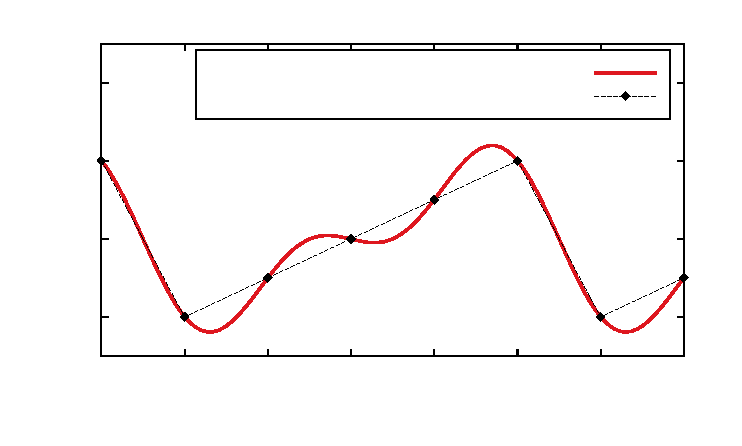
\includegraphics{example-2}}%
    \gplfronttext
  \end{picture}%
\endgroup

				\caption{trigonometrisches Polynom und Stützpunkte der Beispielfunktion $g$ }
				\label{fig:example}
			\end{figure}
			
		% subsection diskrete_fouriertransformation (end)

	% section mathematische_grundlagen (end)

	\section{Serieller Algorithmus} % (fold)
	\label{sec:serieller_algorithmus}

		\subsection{Idee der Fast Fourier Transform} % (fold)
		\label{sub:idee_der_fast_fourier_transform}
		
			Im Folgenden bezeichne $W(n)$ die Anzahl der Operationen (hier $+,\cdot$), die ein gegebener Algorithmus in Abhängigkeit der Eingabegröße $n$ ausführt.

			Für einen naiven Algorithmus, der nach obiger Formel die DFT von $g$ berechnet, gilt nun
			\[ W(n) = \underbrace{n(n+1)}_{\mathclap{\mathrm{Multiplikation}}} + \underbrace{n(n-1)}_{\mathclap{\mathrm{Addition}}} = 2n^2 \in \Omega\curvb{n^2} \]
			Dabei wurde die Berechnung der Faktoren $e^{-i\xi}$, die auch Twiddle-Faktoren genannt werden, nicht beachtet.
			Diese können durch geeignete Tabellenwerte, die dem Programm vorab zur Verfügung gestellt werden, direkt abgelesen werden.
			Die Berechnung muss nun für alle $n$ Koeffizienten durchgeführt werden.

			Um diese Laufzeitkomplexität zu verbessern, teilt man die Berechnung der DFT in gerade und ungerade Summanden ein.
			Es sei nun $n=2m$ für ein $m\in\SN$ und $\FF_n$ bezeichne die DFT auf dem Raum $\SC^n$.
			Für $k\in\mathrm{N}_n$ folgt
			\begin{alignat*}{3}
				\FF_ng(k) &=&& \ \frac{1}{n}\sum_{x=0}^{n-1} g(x)\exp\curvb{ -\frac{2\pi i}{n}kx } \\
				&=&& \ \frac{1}{n} \boxb{ \sum_{x=0}^{m-1} f(2x)e^{-\frac{2\pi i}{n}2kx} + \sum_{x=0}^{m-1} f(2x+1)e^{-\frac{2\pi i}{n}k(2x+1)} } \\
				&=&& \ \frac{1}{2}\boxb{\frac{1}{m} \sum_{x=0}^{m-1} g(2x)e^{-\frac{2\pi i}{m}kx} + e^{-\frac{\pi i}{m}k} \frac{1}{m} \sum_{x=0}^{m-1} g(2x+1)e^{-\frac{2\pi i}{m}kj}}
			\end{alignat*}
			Für $k<m$ können diese beiden Summen durch diskrete Fouriertransformationen für $m$ Punkte ersetzt werden.
			\begin{alignat*}{3}
				g_0:\mathrm{N}_m\longrightarrow\SC,\qquad g_0(x) &:=&& \ g(2x) \\
				g_1:\mathrm{N}_m\longrightarrow\SC,\qquad g_1(x) &:=&& \ g(2x+1)
			\end{alignat*}
			\begin{alignat*}{5}
				&\FF_n g(k) &&=&& \ \frac{1}{2}\curvb{\FF_m g_0(k) + e^{-\frac{\pi i}{m}k} \ \FF_m g_1(k)} \\
				&\FF_n g(k+m) &&=&& \ \frac{1}{2}\curvb{\FF_m g_0(k) - e^{-\frac{\pi i}{m}k} \ \FF_m g_1(k)}
			\end{alignat*}
			% \end{tcolorbox}
			Das Ausführen der Fouriertransformation für $n$ Punkte wird also auf die Ausführung zweier Fouriertransformationen für $n/2$ Punkte zurückgeführt.
			Man möchte nun durch ein rekursives Wiederholen dieser Prozedur die Laufzeitkomplexität verbessern.
			Aus diesem Grund wird nun hier und im Folgenden $n=2^p$ für ein $p\in\SN$ gesetzt.
			Dadurch sind exakt $p$ rekursive Schritte mögliche.

			\begin{proposition*}[Zeitkomplexität]
				Gilt $W(1)=0$ und
				\[ \forall k\in\mathrm{N}_m:\quad W(2k) = 2W(k) + 4k \]
				so folgt für die explizite Darstellung der Zeitkomplexität
				\[ W(n) = 2n\log_2n \in \Omega(n\log_2n) \]
			\end{proposition*}

			Auch bei der angegebenen Proposition werden die Twiddle-Faktoren nicht beachtet.			
			Mithilfe dieses Algorithmus erfährt die Berechnung der DFT eine signifikante Beschleunigung.
			Algorithmen, welche bei der Berechnung der DFT diese Zeitkomplexität aufweisen, werden im allgemeinen Fast Fourier Transform oder auch FFT genannt.

		% subsection idee_der_fast_fourier_transform (end)

		\subsection{Rekursiver Algorithmus} % (fold)
		\label{sub:rekursiver_algorithmus}
		
			Ein erster einfacher FFT-Algorithmus ergibt sich nun direkt aus den oben beschriebenen rekursiven Gleichungen.
			% Dieser Algorithmus arbeitet, wie auch die Gleichungen, durch einen rekursiven Aufruf von sich selbst.
			Um dies in der gegebenen Sprache zu verwirklichen ist eine zusätzliche Prozedur im Programm nötig.

			\begin{tcolorbox}[colframe=black,colbacktitle=white,coltitle=black, attach boxed title to top center={yshift=-2mm},enhanced, titlerule=0.1pt, boxrule=0.5pt, arc=5pt,title=Listing:\quad rekursiver FFT-Algorithmus]
				\begin{tabbing}
	\quad\=\quad\=\quad\=\kill
	$\mathbf{program} \textrm{ Recursive-FFT}$\\
	$\mathbf{declare}$\\
		\>$\mathbf{procedure} \textrm{ fft}(\mathit{out},\mathit{in}\ :\ \mathrm{array}[0..2^{q}-1-1] \textrm{ of complex}\ ;\ q\ :\ \mathrm{integer});$ \\
		\>$t\ :\ \textrm{integer}\ ;$\\
		\>$\omega,b,c\ :\ \mathrm{array}[0..2^{p}-1] \textrm{ of complex}$\\
	$\mathbf{initially}$\\
		\>$\color{MidnightBlue}\curlb{\textit{\ttfamily look-up table for twiddle factors}}$\\
		\>$\langle \ ;\ t\ :\ 0\leq t<2^p\ ::\ \omega[t] = \exp(-\frac{2\pi it}{n})\ \rangle\ ;$\\
		\>$\langle \ ;\ t\ :\ 0\leq t<2^p\ ::\ b[t] = g(t)\ \rangle$\\
	$\mathbf{assign}$\\
		\>$\mathrm{fft}(c,b,p)$\\
	$\mathbf{end}$\\
	% \\
	\\
	$\color{MidnightBlue}\curlb{\textit{\ttfamily extra procedure for recursive algorithm}}$\\
	$\mathbf{procedure} \textrm{ fft}(\mathit{out},\mathit{in}\ :\ \mathrm{array}[0..2^{q}-1-1] \textrm{ of complex}\ ;\ q\ :\ \mathrm{integer})$ \\
	$\mathbf{begin}$\\
		\>$\mathbf{if}\ q=0\ \mathbf{then}$\\
			\>\>$\mathit{out}[0] = \mathit{in}[0]$\\
		\>$\mathbf{else}\ \mathbf{begin}$\\
		% \>$$\\
			\>\>$\mathrm{fft}(\mathit{out}[0..2^{q-1}-1]\ ,\ \mathit{in}[0..2..2^{q}-2]\ ,\ q-1);$\\
			\>\>$\mathrm{fft}(\mathit{out}[2^{q-1}..2^q-1]\ ,\ \mathit{in}[1..2..2^{q}-1]\ ,\ q-1);$\\
			% \\
			\>\>$\langle \ \|\ t\ :\ 0\leq t<2^{q-1}\ ::$\\
				\>\>\>$\boxb{ \begin{array}{l} b[t] \\ b[t+2^{q-1}] \end{array} } := \dfrac{1}{2} \boxb{ \begin{array}{lr} 1 & \omega[2^{p-q}t] \\ 1 & -\omega[2^{p-q}t] \end{array} }\boxb{ \begin{array}{l} b[t] \\ b[t+2^{q-1}] \end{array} }$\\
			\>\>$\rangle$\\
		\>$\mathbf{end}$\\
	$\mathbf{end}$\\
\end{tabbing}



			\end{tcolorbox}

			% \begin{tcolorbox}[colframe=black,colbacktitle=white,coltitle=black, attach boxed title to top center={yshift=-2mm},enhanced, titlerule=0.1pt, boxrule=0.5pt, arc=5pt,title=Listing:\quad rekursiver FFT-Algorithmus Teil 2]
			% 	\begin{tabbing}
	\quad\=\quad\=\quad\=\kill
	$\color{MidnightBlue}\curlb{\textit{\ttfamily extra procedure for recursive algorithm}}$\\
	$\mathbf{procedure} \textrm{ fft}(\mathit{out},\mathit{in}\ :\ \mathrm{array}[0..2^{q}-1-1] \textrm{ of complex}\ ;\ q\ :\ \mathrm{integer})$ \\
	$\mathbf{begin}$\\
		\>$\mathbf{if}\ q=0\ \mathbf{then}$\\
			\>\>$\mathit{out}[0] = \mathit{in}[0]$\\
		\>$\mathbf{else}\ \mathbf{begin}$\\
		% \>$$\\
			\>\>$\mathrm{fft}(\mathit{out}[0..2^{q-1}-1]\ ,\ \mathit{in}[0..2..2^{q}-2]\ ,\ q-1);$\\
			\>\>$\mathrm{fft}(\mathit{out}[2^{q-1}..2^q-1]\ ,\ \mathit{in}[1..2..2^{q}-1]\ ,\ q-1);$\\
			% \\
			\>\>$\langle \ \|\ t\ :\ 0\leq t<2^{q-1}\ ::$\\
				\>\>\>$\boxb{ \begin{array}{l} b[t] \\ b[t+2^{q-1}] \end{array} } := \dfrac{1}{2} \boxb{ \begin{array}{lr} 1 & \omega[2^{p-q}t] \\ 1 & -\omega[2^{p-q}t] \end{array} }\boxb{ \begin{array}{l} b[t] \\ b[t+2^{q-1}] \end{array} }$\\
			\>\>$\rangle$\\
		\>$\mathbf{end}$\\
	$\mathbf{end}$\\
\end{tabbing}
			% \end{tcolorbox}			

		% subsection rekursiver_algorithmus (end)

		\newpage

		\subsection{Von Bit-Reversal zu Butterfly} % (fold)
		\label{sub:von_bit_reversal_zu_butterfly}
		
			Um aus dem oben beschriebenen Algorithmus einen nicht-rekursiven Algorithmus zu erstellen, ist eine genau Analyse nötig.
			Diese soll anhand eines Beispiels veranschaulicht werden.
			Es sei dafür $p=3$ und damit $n=8$.
			Das Eingabearray $b$ besitzt also $8$ Elemente.
			In jedem rekursiven Aufruf werden die Werte von $b$ mit geraden und ungeraden Indizes in zwei neue Eingabearrays aufgespalten.
			Dies wird solange wiederholt, bis die Länge des Eingabearrays $1$ beträgt.
			Am Ende wird dann nur noch auf einem permutierten Array $\tilde{b}$ mit $\tilde{b}[t]:=b[\sigma_p(t)]$ gearbeitet.
			Abbildung \ref{fig:bit-reversal} veranschaulicht dies.
			Stellt man nun alle Indizes im Binärformat mit $p$ Stellen dar, so ergibt sich zum Beispiel
			\begin{alignat*}{3}
				0 = (000)_2 \quad\stackrel{\sigma_p}{\longrightarrow}\quad 0 = (000)_2 \\
				1 = (001)_2 \quad\stackrel{\sigma_p}{\longrightarrow}\quad 4 = (100)_2 \\
				2 = (010)_2 \quad\stackrel{\sigma_p}{\longrightarrow}\quad 2 = (010)_2 \\
				3 = (011)_2 \quad\stackrel{\sigma_p}{\longrightarrow}\quad 6 = (110)_2 \\
				4 = (100)_2 \quad\stackrel{\sigma_p}{\longrightarrow}\quad 1 = (001)_2 \\
				5 = (101)_2 \quad\stackrel{\sigma_p}{\longrightarrow}\quad 5 = (101)_2 \\
				6 = (110)_2 \quad\stackrel{\sigma_p}{\longrightarrow}\quad 3 = (011)_2 \\
				7 = (111)_2 \quad\stackrel{\sigma_p}{\longrightarrow}\quad 7 = (111)_2
			\end{alignat*}
			Die Binärdarstellungen der Indizes wird also gerade umgekehrt.
			Dies gilt nicht nur für den Spezialfall $p=3$, sonder für alle $p$.

			\begin{proposition*}[Bit-Reversal Map]
				Sei $t\in\mathrm{N}_{2^p}$ mit der Binärdarstellung $(\alpha_{p-1}\ldots\alpha_0)_2$.
				Dann ergibt sich nach obigen Definitionen für die Binärdarstellung von $\sigma_p(t)$
				\[ (\alpha_0\ldots\alpha_{p-1})_2 \]
				$\sigma_p$ wird dann auch als Bit-Reversal Map bezeichnet.
			\end{proposition*}

			\begin{figure}[p]
				\center
				\unitlength1cm
\begin{picture}(9,9)(-1,-3)
	\put(-0.1,5){$b_0$}
	\put(0.9,5){$b_1$}
	\put(1.9,5){$b_2$}
	\put(2.9,5){$b_3$}
	\put(3.9,5){$b_4$}
	\put(4.9,5){$b_5$}
	\put(5.9,5){$b_6$}
	\put(6.9,5){$b_7$}

	\put(-0.1,3){$b_0$}
	\put(0.9,3){$b_2$}
	\put(1.9,3){$b_4$}
	\put(2.9,3){$b_6$}
	\put(3.9,3){$b_1$}
	\put(4.9,3){$b_3$}
	\put(5.9,3){$b_5$}
	\put(6.9,3){$b_7$}

	\put(-0.1,1){$b_0$}
	\put(0.9,1){$b_4$}
	\put(1.9,1){$b_2$}
	\put(2.9,1){$b_6$}
	\put(3.9,1){$b_1$}
	\put(4.9,1){$b_5$}
	\put(5.9,1){$b_3$}
	\put(6.9,1){$b_7$}

	\put(-0.1,-1){$b_0$}
	\put(0.9,-1){$b_4$}
	\put(1.9,-1){$b_2$}
	\put(2.9,-1){$b_6$}
	\put(3.9,-1){$b_1$}
	\put(4.9,-1){$b_5$}
	\put(5.9,-1){$b_3$}
	\put(6.9,-1){$b_7$}

	\put(-0.1,-2.4){$\tilde{b}_0$}
	\put(0.9,-2.4){$\tilde{b}_1$}
	\put(1.9,-2.4){$\tilde{b}_2$}
	\put(2.9,-2.4){$\tilde{b}_3$}
	\put(3.9,-2.4){$\tilde{b}_4$}
	\put(4.9,-2.4){$\tilde{b}_5$}
	\put(5.9,-2.4){$\tilde{b}_6$}
	\put(6.9,-2.4){$\tilde{b}_7$}

	\put(-0.1,-1.8){\rotatebox{90}{$:=$}}
	\put(0.9,-1.8){\rotatebox{90}{$:=$}}
	\put(1.9,-1.8){\rotatebox{90}{$:=$}}
	\put(2.9,-1.8){\rotatebox{90}{$:=$}}
	\put(3.9,-1.8){\rotatebox{90}{$:=$}}
	\put(4.9,-1.8){\rotatebox{90}{$:=$}}
	\put(5.9,-1.8){\rotatebox{90}{$:=$}}
	\put(6.9,-1.8){\rotatebox{90}{$:=$}}

	\put(0,4.6){\vector(0,-1){1}}
	\put(1,4.6){\vector(3,-1){3}}
	\put(2,4.6){\vector(-1,-1){1}}
	\put(3,4.6){\vector(2,-1){2}}
	\put(4,4.6){\vector(-2,-1){2}}
	\put(5,4.6){\vector(1,-1){1}}
	\put(6,4.6){\vector(-3,-1){3}}
	\put(7,4.6){\vector(0,-1){1}}

	\put(0,2.6){\vector(0,-1){1}}
	\put(1,2.6){\vector(1,-1){1}}
	\put(2,2.6){\vector(-1,-1){1}}
	\put(3,2.6){\vector(0,-1){1}}
	\put(4,2.6){\vector(0,-1){1}}
	\put(5,2.6){\vector(1,-1){1}}
	\put(6,2.6){\vector(-1,-1){1}}
	\put(7,2.6){\vector(0,-1){1}}

	\put(0,0.6){\vector(0,-1){1}}
	\put(1,0.6){\vector(0,-1){1}}
	\put(2,0.6){\vector(0,-1){1}}
	\put(3,0.6){\vector(0,-1){1}}
	\put(4,0.6){\vector(0,-1){1}}
	\put(5,0.6){\vector(0,-1){1}}
	\put(6,0.6){\vector(0,-1){1}}
	\put(7,0.6){\vector(0,-1){1}}

	\put(-0.3,4.7){\dashbox{0.1}(7.6,0.8)}

	\put(-0.3,2.7){\dashbox{0.1}(3.6,0.8)}
	\put(3.7,2.7){\dashbox{0.1}(3.6,0.8)}

	\put(-0.3,0.7){\dashbox{0.1}(1.6,0.8)}
	\put(1.7,0.7){\dashbox{0.1}(1.6,0.8)}
	\put(3.7,0.7){\dashbox{0.1}(1.6,0.8)}
	\put(5.7,0.7){\dashbox{0.1}(1.6,0.8)}

	\put(-0.3,-1.3){\dashbox{0.1}(0.6,0.8)}
	\put(0.7,-1.3){\dashbox{0.1}(0.6,0.8)}
	\put(1.7,-1.3){\dashbox{0.1}(0.6,0.8)}
	\put(2.7,-1.3){\dashbox{0.1}(0.6,0.8)}
	\put(3.7,-1.3){\dashbox{0.1}(0.6,0.8)}
	\put(4.7,-1.3){\dashbox{0.1}(0.6,0.8)}
	\put(5.7,-1.3){\dashbox{0.1}(0.6,0.8)}
	\put(6.7,-1.3){\dashbox{0.1}(0.6,0.8)}

	\put(-0.3,-2.7){\dashbox{0.1}(7.6,0.8)}
\end{picture}
				\caption{Bit-Reversal Map: \\ Funktionsweise des rekursiven FFT-Algorithmus bis zum Erreichen der Abbruchbedingung für $p=3$}
				\label{fig:bit-reversal}
			\end{figure}

			Der zweite Teil des rekursiven Algorithmus lässt sich durch Abbildung \ref{fig:butterfly} veranschaulichen.
			Nachdem alle Instanzen der Prozedur aufgerufen wurden, muss jetzt das Matrix-Vektor-Produkt berechnet werden.
			Die einzelnen $+$ in der Abbildung stehen für die Berechnung der ersten Zeile.
			Die einzelnen $-$ stehen also für die zweite Zeile.
			Dieses Schema wird auch Schmetterlingsgraph oder Butterfly Graph genannt.

			\begin{figure}[p]
				\center
				\unitlength1cm
\begin{picture}(9,8)(-1,-2)
	\put(-0.1,5){$c_0$}
	\put(0.9,5){$c_1$}
	\put(1.9,5){$c_2$}
	\put(2.9,5){$c_3$}
	\put(3.9,5){$c_4$}
	\put(4.9,5){$c_5$}
	\put(5.9,5){$c_6$}
	\put(6.9,5){$c_7$}

	\put(-0.1,3){$c_0$}
	\put(0.9,3){$c_1$}
	\put(1.9,3){$c_2$}
	\put(2.9,3){$c_3$}
	\put(3.9,3){$c_4$}
	\put(4.9,3){$c_5$}
	\put(5.9,3){$c_6$}
	\put(6.9,3){$c_7$}

	\put(-0.1,3.15){$^+$}
	\put(0.9,3.15){$^-$}
	\put(1.9,3.15){$^+$}
	\put(2.9,3.15){$^-$}
	\put(3.9,3.15){$^+$}
	\put(4.9,3.15){$^-$}
	\put(5.9,3.15){$^+$}
	\put(6.9,3.15){$^-$}

	\put(-0.1,1){$c_0$}
	\put(0.9,1){$c_1$}
	\put(1.9,1){$c_2$}
	\put(2.9,1){$c_3$}
	\put(3.9,1){$c_4$}
	\put(4.9,1){$c_5$}
	\put(5.9,1){$c_6$}
	\put(6.9,1){$c_7$}

	\put(-0.1,1.15){$^+$}
	\put(0.9,1.15){$^+$}
	\put(1.9,1.15){$^-$}
	\put(2.9,1.15){$^-$}
	\put(3.9,1.15){$^+$}
	\put(4.9,1.15){$^+$}
	\put(5.9,1.15){$^-$}
	\put(6.9,1.15){$^-$}

	\put(-0.1,-1){$c_0$}
	\put(0.9,-1){$c_1$}
	\put(1.9,-1){$c_2$}
	\put(2.9,-1){$c_3$}
	\put(3.9,-1){$c_4$}
	\put(4.9,-1){$c_5$}
	\put(5.9,-1){$c_6$}
	\put(6.9,-1){$c_7$}

	\put(-0.1,-0.85){$^+$}
	\put(0.9,-0.85){$^+$}
	\put(1.9,-0.85){$^+$}
	\put(2.9,-0.85){$^+$}
	\put(3.9,-0.85){$^-$}
	\put(4.9,-0.85){$^-$}
	\put(5.9,-0.85){$^-$}
	\put(6.9,-0.85){$^-$}

	% \put(-0.1,-2.4){$\tilde{b}_0$}
	% \put(0.9,-2.4){$\tilde{b}_1$}
	% \put(1.9,-2.4){$\tilde{b}_2$}
	% \put(2.9,-2.4){$\tilde{b}_3$}
	% \put(3.9,-2.4){$\tilde{b}_4$}
	% \put(4.9,-2.4){$\tilde{b}_5$}
	% \put(5.9,-2.4){$\tilde{b}_6$}
	% \put(6.9,-2.4){$\tilde{b}_7$}

	% \put(-0.1,-1.8){\rotatebox{90}{$:=$}}
	% \put(0.9,-1.8){\rotatebox{90}{$:=$}}
	% \put(1.9,-1.8){\rotatebox{90}{$:=$}}
	% \put(2.9,-1.8){\rotatebox{90}{$:=$}}
	% \put(3.9,-1.8){\rotatebox{90}{$:=$}}
	% \put(4.9,-1.8){\rotatebox{90}{$:=$}}
	% \put(5.9,-1.8){\rotatebox{90}{$:=$}}
	% \put(6.9,-1.8){\rotatebox{90}{$:=$}}

	\put(0,4.6){\vector(0,-1){1}}
	\put(1,4.6){\vector(0,-1){1}}
	\put(2,4.6){\vector(0,-1){1}}
	\put(3,4.6){\vector(0,-1){1}}
	\put(4,4.6){\vector(0,-1){1}}
	\put(5,4.6){\vector(0,-1){1}}
	\put(6,4.6){\vector(0,-1){1}}
	\put(7,4.6){\vector(0,-1){1}}

	\put(0,4.6){\vector(1,-1){1}}
	\put(2,4.6){\vector(1,-1){1}}
	\put(4,4.6){\vector(1,-1){1}}
	\put(6,4.6){\vector(1,-1){1}}
	\put(1,4.6){\vector(-1,-1){1}}
	\put(3,4.6){\vector(-1,-1){1}}
	\put(5,4.6){\vector(-1,-1){1}}
	\put(7,4.6){\vector(-1,-1){1}}

	\put(0,2.6){\vector(0,-1){1}}
	\put(1,2.6){\vector(0,-1){1}}
	\put(2,2.6){\vector(0,-1){1}}
	\put(3,2.6){\vector(0,-1){1}}
	\put(4,2.6){\vector(0,-1){1}}
	\put(5,2.6){\vector(0,-1){1}}
	\put(6,2.6){\vector(0,-1){1}}
	\put(7,2.6){\vector(0,-1){1}}

	\put(0,2.6){\vector(2,-1){2}}
	\put(1,2.6){\vector(2,-1){2}}
	\put(4,2.6){\vector(2,-1){2}}
	\put(5,2.6){\vector(2,-1){2}}
	\put(2,2.6){\vector(-2,-1){2}}
	\put(3,2.6){\vector(-2,-1){2}}
	\put(6,2.6){\vector(-2,-1){2}}
	\put(7,2.6){\vector(-2,-1){2}}

	\put(0,0.6){\vector(0,-1){1}}
	\put(1,0.6){\vector(0,-1){1}}
	\put(2,0.6){\vector(0,-1){1}}
	\put(3,0.6){\vector(0,-1){1}}
	\put(4,0.6){\vector(0,-1){1}}
	\put(5,0.6){\vector(0,-1){1}}
	\put(6,0.6){\vector(0,-1){1}}
	\put(7,0.6){\vector(0,-1){1}}

	\put(0,0.6){\vector(4,-1){4}}
	\put(1,0.6){\vector(4,-1){4}}
	\put(2,0.6){\vector(4,-1){4}}
	\put(3,0.6){\vector(4,-1){4}}
	\put(4,0.6){\vector(-4,-1){4}}
	\put(5,0.6){\vector(-4,-1){4}}
	\put(6,0.6){\vector(-4,-1){4}}
	\put(7,0.6){\vector(-4,-1){4}}


	% \put(0,4.6){\vector(0,-1){1}}
	% \put(1,4.6){\vector(3,-1){3}}
	% \put(2,4.6){\vector(-1,-1){1}}
	% \put(3,4.6){\vector(2,-1){2}}
	% \put(4,4.6){\vector(-2,-1){2}}
	% \put(5,4.6){\vector(1,-1){1}}
	% \put(6,4.6){\vector(-3,-1){3}}
	% \put(7,4.6){\vector(0,-1){1}}

	% \put(0,2.6){\vector(0,-1){1}}
	% \put(1,2.6){\vector(1,-1){1}}
	% \put(2,2.6){\vector(-1,-1){1}}
	% \put(3,2.6){\vector(0,-1){1}}
	% \put(4,2.6){\vector(0,-1){1}}
	% \put(5,2.6){\vector(1,-1){1}}
	% \put(6,2.6){\vector(-1,-1){1}}
	% \put(7,2.6){\vector(0,-1){1}}

	

	\put(-0.3,-1.3){\dashbox{0.1}(7.6,0.8)}

	\put(-0.3,0.7){\dashbox{0.1}(3.6,0.8)}
	\put(3.7,0.7){\dashbox{0.1}(3.6,0.8)}

	\put(-0.3,2.7){\dashbox{0.1}(1.6,0.8)}
	\put(1.7,2.7){\dashbox{0.1}(1.6,0.8)}
	\put(3.7,2.7){\dashbox{0.1}(1.6,0.8)}
	\put(5.7,2.7){\dashbox{0.1}(1.6,0.8)}

	\put(-0.3,4.7){\dashbox{0.1}(0.6,0.8)}
	\put(0.7,4.7){\dashbox{0.1}(0.6,0.8)}
	\put(1.7,4.7){\dashbox{0.1}(0.6,0.8)}
	\put(2.7,4.7){\dashbox{0.1}(0.6,0.8)}
	\put(3.7,4.7){\dashbox{0.1}(0.6,0.8)}
	\put(4.7,4.7){\dashbox{0.1}(0.6,0.8)}
	\put(5.7,4.7){\dashbox{0.1}(0.6,0.8)}
	\put(6.7,4.7){\dashbox{0.1}(0.6,0.8)}

	% \put(-0.3,-2.7){\dashbox{0.1}(7.6,0.8)}
\end{picture}
				\caption{Butterfly Graph: \\ Funktionsweise des rekursiven FFT-Algorithmus nach dem Erreichen der Abbruchbedingung für $p=3$}
				\label{fig:butterfly}
			\end{figure}

		% subsection von_bit_reversal_zu_butterfly (end)

		\newpage

		\subsection{Nicht-Rekursiver Algorithmus} % (fold)
		\label{sub:nicht_rekursiver_algorithmus}
		
			Durch die oben beschriebene Analyse führt nun auf den folgenden nicht-rekursiven Algorithmus.

			\begin{tcolorbox}[colframe=black,colbacktitle=white,coltitle=black, attach boxed title to top center={yshift=-2mm},enhanced, titlerule=0.1pt, boxrule=0.5pt, arc=5pt,title=Listing:\quad nicht-rekursiver FFT-Algorithmus]
				\begin{tabbing}
	\quad\=\quad\=\quad\=\kill
	$\mathbf{program} \textrm{ Serial-FFT}$\\
	$\mathbf{declare}$\\
		% \>$\mathbf{procedure} \textrm{ fft}(\mathit{out},\mathit{in}\ :\ \mathrm{array}[0..2^{q}-1-1] \textrm{ of complex}\ ;\ q\ :\ \mathrm{integer});$ \\
		\>$m,t\ :\ \textrm{integer}\ ;$\\
		\>$\omega,b\ :\ \mathrm{array}[0..2^{p}-1] \textrm{ of complex}$\\
	$\mathbf{initially}$\\
		\>$\color{MidnightBlue}\curlb{\textit{\ttfamily look-up table for twiddle factors}}$\\
		\>$\langle \ ;\ t\ :\ 0\leq t<2^p\ ::\ \omega[t] = \exp(-\frac{2\pi it}{n})\ \rangle\ ;$\\
		\>$\color{MidnightBlue}\curlb{\textit{\ttfamily bit-reverse ordering}}$\\
		\>$\langle \ ;\ t\ :\ 0\leq t<2^p\ ::\ b[t] = g(\sigma_p(t))\ \rangle$\\
	$\mathbf{assign}$\\
		% \>$\mathrm{fft}(c,b,p)$\\
		\>$\color{MidnightBlue}\curlb{\textit{\ttfamily butterfly calculation}}$\\
		\>$\langle \ ;\ m\ :\ 0\leq m<p\ ::$\\
			\>\>$\langle \ \|\ t\ :\ 0\leq t<2^{p}-1\ \mathbf{and}\ t\wedge 2^m=0\ ::$\\
				\>\>\>$\boxb{ \begin{array}{l} b[t] \\ b[t+2^m] \end{array} } := \dfrac{1}{2} \boxb{ \begin{array}{lr} 1 & \omega[2^{p-m-1}t\ \mathrm{mod}\ 2^{p-1}] \\ 1 & -\omega[2^{p-m-1}t\ \mathrm{mod}\ 2^{p-1}] \end{array} }\boxb{ \begin{array}{l} b[t] \\ b[t+2^m] \end{array} }$\\
			\>\>$\rangle$\\
		\>$\rangle$\\
	$\mathbf{end}$\\
	% \\
	% \\
	% $\mathbf{procedure} \textrm{ fft}(\mathit{out},\mathit{in}\ :\ \mathrm{array}[0..2^{q}-1-1] \textrm{ of complex}\ ;\ q\ :\ \mathrm{integer})$ \\
	% $\mathbf{begin}$\\
	% 	\>$\mathbf{if}\ q=0\ \mathbf{then}$\\
	% 		\>\>$\mathit{out}[0] = \mathit{in}[0]$\\
	% 	\>$\mathbf{else}$\\
	% 	\>$\mathbf{begin}$\\
	% 		\>\>$\mathrm{fft}(\mathit{out}[0..2^{q-1}-1]\ ,\ \mathit{in}[0..2..2^{q}-2]\ ,\ q-1);$\\
	% 		\>\>$\mathrm{fft}(\mathit{out}[2^{q-1}..2^q-1]\ ,\ \mathit{in}[1..2..2^{q}-1]\ ,\ q-1);$\\
	% 		\\
	% 		\>\>$\langle \ \|\ t\ :\ 0\leq t<2^{q-1}\ ::$\\
	% 			\>\>\>$\boxb{ \begin{array}{l} b[t] \\ b[t+2^{q-1}] \end{array} } := \dfrac{1}{2} \boxb{ \begin{array}{lr} 1 & \omega[2^{p-q}t] \\ 1 & -\omega[2^{p-q}t] \end{array} }\boxb{ \begin{array}{l} b[t] \\ b[t+2^{q-1}] \end{array} }$\\
	% 		\>\>$\rangle$\\
	% 	\>$\mathbf{end}$\\
	% $\mathbf{end}$\\
\end{tabbing}
			\end{tcolorbox}

		% subsection nicht_rekursiver_algorithmus (end)

	% section serieller_algorithmus (end)

	\section{Paralleler Algorithmus} % (fold)
	\label{sec:paralleler_algorithmus}
	
		\subsection{Verteilung der Daten} % (fold)
		\label{sub:verteilung_der_daten}

			Die Länge des Eingabearrays beträgt $n=2^p$.
			Will man nun den nicht-rekursiven Algorithmus parallelisieren, so ist es durchaus sinnvoll für die Anzahl der Prozesse ebenfalls eine Potenz von $2$ zu verwenden.
			Es sei also $P=2^q$ für ein $q\in\SN$ mit $q\leq p$ die Anzahl der Prozesse.
			Um die Arbeit nun möglichst gleichmäßig zu verteilen, soll nun jeder Prozess gerade $2^{p-q}$ Elemente speichern.
			Abbildung \ref{fig:data-distribution} stellt diese Verteilung für $p=3$ und $q=2$ dar.

			\begin{figure}[h]
				\center
				\unitlength1cm
\begin{picture}(9,2)(-1,0)
	\put(-0.1,1){$\tilde{b}_0$}
	\put(0.9,1){$\tilde{b}_1$}
	\put(1.9,1){$\tilde{b}_2$}
	\put(2.9,1){$\tilde{b}_3$}
	\put(3.9,1){$\tilde{b}_4$}
	\put(4.9,1){$\tilde{b}_5$}
	\put(5.9,1){$\tilde{b}_6$}
	\put(6.9,1){$\tilde{b}_7$}

	\put(-0.3,0.7){\framebox(1.6,0.8)}
	\put(1.7,0.7){\framebox(1.6,0.8)}
	\put(3.7,0.7){\framebox(1.6,0.8)}
	\put(5.7,0.7){\framebox(1.6,0.8)}

	\put(0.4,0.3){$\rho_0$}
	\put(2.4,0.3){$\rho_1$}
	\put(4.4,0.3){$\rho_2$}
	\put(6.4,0.3){$\rho_3$}
\end{picture}
				\caption{Verteilung des Eingabearrays $\tilde{b}$ auf den Prozessen $\rho_i$ für $p=3,q=2$}
				\label{fig:data-distribution}
			\end{figure}

			Damit reichen die lokalen Indizes des Arrays $\tilde{b}$ bezüglich eines Prozesses von $0$ bis $2^{p-q}-1$.
			Ein globaler Index $u\in\mathrm{N}_{2^p}$ bezüglich eines Prozessindex $v\in\mathrm{N}_{2^q}$ und eines lokalen Index $w\in\mathrm{N}_{2^{p-q}}$ ergibt sich dann zu
			\[ u = 2^{p-q}v + w \]
			Bezeichnet man die zugehörigen Binärdarstellungen mit $(u_p\ldots u_1)_2, (v_q\ldots v_1)_2$ und $(w_{p-q}\ldots w_1)_2$ so folgt dann
			\[ (u_p\ldots u_1)_2 = (v_q\ldots v_1 w_{p-q}\ldots w_1)_2 \]
			Die ersten $q$ Bits des globalen Index bezeichnen den Prozessindex und die Restlichen den lokalen Index bezüglich dieses Prozesses.

		
		% subsection verteilung_der_daten (end)

		\subsection{Kommunikation und Algorithmus} % (fold)
		\label{sub:kommunikation_und_algorithmus}

			Man wendet jetzt den Butterfly-Algorithmus auf diese Datenverteilung an (siehe Abbildung \ref{fig:butterfly-parallel}).
			Es gibt dann Teilschritte, die keine Kommunikation zwischen den Prozessen benötigen.
			Für diese Schritte benötigen die Berechnungen nur Werte des eigenen Prozesses.
			Dies gilt für alle $m\in\SN_0$ mit $m<p-q$, sofern die $m$ die im Algorithmus beschriebene Zählvariable bezeichnet.

			Für alle anderen Schritte muss ein Prozess immer genau mit einem anderen kommunizieren.
			Hierbei muss jeder Prozess alle lokal gespeicherten Werte versenden und alle gespeicherten Werte des anderen Prozesses empfangen.
			Dann kann prinzipiell wieder das Matrix-Vektor-Produkt berechnet werden.
			Allerdings muss darauf geachtet werden, dass jeweils eine Zeile durch einen Prozess berechnet wird.

			\begin{figure}[h]
				\center
				\unitlength1cm
\begin{picture}(9,8)(-1,-2)
	\put(-0.1,5){$b_0$}
	\put(0.9,5){$b_1$}
	\put(1.9,5){$b_2$}
	\put(2.9,5){$b_3$}
	\put(3.9,5){$b_4$}
	\put(4.9,5){$b_5$}
	\put(5.9,5){$b_6$}
	\put(6.9,5){$b_7$}

	\put(-0.1,3){$b_0$}
	\put(0.9,3){$b_1$}
	\put(1.9,3){$b_2$}
	\put(2.9,3){$b_3$}
	\put(3.9,3){$b_4$}
	\put(4.9,3){$b_5$}
	\put(5.9,3){$b_6$}
	\put(6.9,3){$b_7$}

	\put(-0.1,3.15){$^+$}
	\put(0.9,3.15){$^-$}
	\put(1.9,3.15){$^+$}
	\put(2.9,3.15){$^-$}
	\put(3.9,3.15){$^+$}
	\put(4.9,3.15){$^-$}
	\put(5.9,3.15){$^+$}
	\put(6.9,3.15){$^-$}

	\put(-0.1,1){$b_0$}
	\put(0.9,1){$b_1$}
	\put(1.9,1){$b_2$}
	\put(2.9,1){$b_3$}
	\put(3.9,1){$b_4$}
	\put(4.9,1){$b_5$}
	\put(5.9,1){$b_6$}
	\put(6.9,1){$b_7$}

	\put(-0.1,1.15){$^+$}
	\put(0.9,1.15){$^+$}
	\put(1.9,1.15){$^-$}
	\put(2.9,1.15){$^-$}
	\put(3.9,1.15){$^+$}
	\put(4.9,1.15){$^+$}
	\put(5.9,1.15){$^-$}
	\put(6.9,1.15){$^-$}

	\put(-0.1,-1){$b_0$}
	\put(0.9,-1){$b_1$}
	\put(1.9,-1){$b_2$}
	\put(2.9,-1){$b_3$}
	\put(3.9,-1){$b_4$}
	\put(4.9,-1){$b_5$}
	\put(5.9,-1){$b_6$}
	\put(6.9,-1){$b_7$}

	\put(-0.1,-0.85){$^+$}
	\put(0.9,-0.85){$^+$}
	\put(1.9,-0.85){$^+$}
	\put(2.9,-0.85){$^+$}
	\put(3.9,-0.85){$^-$}
	\put(4.9,-0.85){$^-$}
	\put(5.9,-0.85){$^-$}
	\put(6.9,-0.85){$^-$}

	% \put(-0.1,-2.4){$\tilde{b}_0$}
	% \put(0.9,-2.4){$\tilde{b}_1$}
	% \put(1.9,-2.4){$\tilde{b}_2$}
	% \put(2.9,-2.4){$\tilde{b}_3$}
	% \put(3.9,-2.4){$\tilde{b}_4$}
	% \put(4.9,-2.4){$\tilde{b}_5$}
	% \put(5.9,-2.4){$\tilde{b}_6$}
	% \put(6.9,-2.4){$\tilde{b}_7$}

	% \put(-0.1,-1.8){\rotatebox{90}{$:=$}}
	% \put(0.9,-1.8){\rotatebox{90}{$:=$}}
	% \put(1.9,-1.8){\rotatebox{90}{$:=$}}
	% \put(2.9,-1.8){\rotatebox{90}{$:=$}}
	% \put(3.9,-1.8){\rotatebox{90}{$:=$}}
	% \put(4.9,-1.8){\rotatebox{90}{$:=$}}
	% \put(5.9,-1.8){\rotatebox{90}{$:=$}}
	% \put(6.9,-1.8){\rotatebox{90}{$:=$}}

	\put(0,4.6){\vector(0,-1){1}}
	\put(1,4.6){\vector(0,-1){1}}
	\put(2,4.6){\vector(0,-1){1}}
	\put(3,4.6){\vector(0,-1){1}}
	\put(4,4.6){\vector(0,-1){1}}
	\put(5,4.6){\vector(0,-1){1}}
	\put(6,4.6){\vector(0,-1){1}}
	\put(7,4.6){\vector(0,-1){1}}

	\put(0,4.6){\vector(1,-1){1}}
	\put(2,4.6){\vector(1,-1){1}}
	\put(4,4.6){\vector(1,-1){1}}
	\put(6,4.6){\vector(1,-1){1}}
	\put(1,4.6){\vector(-1,-1){1}}
	\put(3,4.6){\vector(-1,-1){1}}
	\put(5,4.6){\vector(-1,-1){1}}
	\put(7,4.6){\vector(-1,-1){1}}

	\put(0,2.6){\vector(0,-1){1}}
	\put(1,2.6){\vector(0,-1){1}}
	\put(2,2.6){\vector(0,-1){1}}
	\put(3,2.6){\vector(0,-1){1}}
	\put(4,2.6){\vector(0,-1){1}}
	\put(5,2.6){\vector(0,-1){1}}
	\put(6,2.6){\vector(0,-1){1}}
	\put(7,2.6){\vector(0,-1){1}}

	\put(0,2.6){\vector(2,-1){2}}
	\put(1,2.6){\vector(2,-1){2}}
	\put(4,2.6){\vector(2,-1){2}}
	\put(5,2.6){\vector(2,-1){2}}
	\put(2,2.6){\vector(-2,-1){2}}
	\put(3,2.6){\vector(-2,-1){2}}
	\put(6,2.6){\vector(-2,-1){2}}
	\put(7,2.6){\vector(-2,-1){2}}

	\put(0,0.6){\vector(0,-1){1}}
	\put(1,0.6){\vector(0,-1){1}}
	\put(2,0.6){\vector(0,-1){1}}
	\put(3,0.6){\vector(0,-1){1}}
	\put(4,0.6){\vector(0,-1){1}}
	\put(5,0.6){\vector(0,-1){1}}
	\put(6,0.6){\vector(0,-1){1}}
	\put(7,0.6){\vector(0,-1){1}}

	\put(0,0.6){\vector(4,-1){4}}
	\put(1,0.6){\vector(4,-1){4}}
	\put(2,0.6){\vector(4,-1){4}}
	\put(3,0.6){\vector(4,-1){4}}
	\put(4,0.6){\vector(-4,-1){4}}
	\put(5,0.6){\vector(-4,-1){4}}
	\put(6,0.6){\vector(-4,-1){4}}
	\put(7,0.6){\vector(-4,-1){4}}


	% \put(0,4.6){\vector(0,-1){1}}
	% \put(1,4.6){\vector(3,-1){3}}
	% \put(2,4.6){\vector(-1,-1){1}}
	% \put(3,4.6){\vector(2,-1){2}}
	% \put(4,4.6){\vector(-2,-1){2}}
	% \put(5,4.6){\vector(1,-1){1}}
	% \put(6,4.6){\vector(-3,-1){3}}
	% \put(7,4.6){\vector(0,-1){1}}

	% \put(0,2.6){\vector(0,-1){1}}
	% \put(1,2.6){\vector(1,-1){1}}
	% \put(2,2.6){\vector(-1,-1){1}}
	% \put(3,2.6){\vector(0,-1){1}}
	% \put(4,2.6){\vector(0,-1){1}}
	% \put(5,2.6){\vector(1,-1){1}}
	% \put(6,2.6){\vector(-1,-1){1}}
	% \put(7,2.6){\vector(0,-1){1}}

	\color{Red}
	% \linethickness{0.3mm}
	\thicklines

	\put(-0.4,-1.4){\dashbox{0.2}(7.8,1)}

	\put(-0.4,0.6){\dashbox{0.2}(3.8,1)}
	\put(3.6,0.6){\dashbox{0.2}(3.8,1)}

	\put(-0.4,2.6){\dashbox{0.2}(1.8,1)}
	\put(1.6,2.6){\dashbox{0.2}(1.8,1)}
	\put(3.6,2.6){\dashbox{0.2}(1.8,1)}
	\put(5.6,2.6){\dashbox{0.2}(1.8,1)}

	\put(-0.4,4.6){\dashbox{0.2}(0.8,1)}
	\put(0.6,4.6){\dashbox{0.2}(0.8,1)}
	\put(1.6,4.6){\dashbox{0.2}(0.8,1)}
	\put(2.6,4.6){\dashbox{0.2}(0.8,1)}
	\put(3.6,4.6){\dashbox{0.2}(0.8,1)}
	\put(4.6,4.6){\dashbox{0.2}(0.8,1)}
	\put(5.6,4.6){\dashbox{0.2}(0.8,1)}
	\put(6.6,4.6){\dashbox{0.2}(0.8,1)}


	\color{Black}
	\thinlines
	% \linethickness{0.3mm}

	\put(-0.3,4.7){\framebox(1.6,0.8)}
	\put(1.7,4.7){\framebox(1.6,0.8)}
	\put(3.7,4.7){\framebox(1.6,0.8)}
	\put(5.7,4.7){\framebox(1.6,0.8)}

	\put(-0.3,2.7){\framebox(1.6,0.8)}
	\put(1.7,2.7){\framebox(1.6,0.8)}
	\put(3.7,2.7){\framebox(1.6,0.8)}
	\put(5.7,2.7){\framebox(1.6,0.8)}

	\put(-0.3,0.7){\framebox(1.6,0.8)}
	\put(1.7,0.7){\framebox(1.6,0.8)}
	\put(3.7,0.7){\framebox(1.6,0.8)}
	\put(5.7,0.7){\framebox(1.6,0.8)}

	\put(-0.3,-1.3){\framebox(1.6,0.8)}
	\put(1.7,-1.3){\framebox(1.6,0.8)}
	\put(3.7,-1.3){\framebox(1.6,0.8)}
	\put(5.7,-1.3){\framebox(1.6,0.8)}

	% \put(-0.3,-2.7){\dashbox{0.1}(7.6,0.8)}
\end{picture}
				\caption{Funktionsweise eines Butterfly Graph auf mehreren Prozessen am Beispiel von $p=3,q=2$}
				\label{fig:butterfly-parallel}
			\end{figure}

			Im folgenden Algorithmus wurde der Zugriff auf die Twiddle-Faktoren abkürzend durch $\xi(m,p,t)$ beschrieben, da die Verteilung solcher Faktoren im Allgemeinen beliebig sein kann.

			\begin{tcolorbox}[colframe=black,colbacktitle=white,coltitle=black, attach boxed title to top center={yshift=-2mm},enhanced, titlerule=0.1pt, boxrule=0.5pt, arc=5pt,title=Listing:\quad paralleler FFT-Algorithmus]
				\begin{tabbing}
	\quad\=\quad\=\quad\=\quad\=\kill
	$0..2^q-1\ \|\ \rho\ \mathbf{program} \textrm{ Parallel-FFT}$\\
	$\mathbf{declare}$\\
		% \>$\mathbf{procedure} \textrm{ fft}(\mathit{out},\mathit{in}\ :\ \mathrm{array}[0..2^{q}-1-1] \textrm{ of complex}\ ;\ q\ :\ \mathrm{integer});$ \\
		\>$m,t\ :\ \textrm{integer}\ ;$\\
		\>$\omega\ :\ \mathrm{array}[0..2^{p}-1] \textrm{ of complex}\ ;$\\
		\>$b,x\ :\ \mathrm{array}[0..2^{p-q}-1] \textrm{ of complex}$\\
	$\mathbf{initially}$\\
		\>$\color{MidnightBlue}\curlb{\textit{\ttfamily look-up table for twiddle factors}}$\\
		\>$\langle \ ;\ t\ :\ 0\leq t<2^p\ ::\ \omega[t] = \exp(-\frac{2\pi it}{n})\ \rangle\ ;$\\
		\>$\color{MidnightBlue}\curlb{\textit{\ttfamily bit-reverse ordering}}$\\
		\>$\langle \ ;\ t\ :\ 0\leq t<2^{p-q}\ ::\ b[t] = g(\sigma_p(2^{p-q}\rho + t))\ \rangle$\\
	$\mathbf{assign}$\\
		% \>$\mathrm{fft}(c,b,p)$\\
		\>$\color{MidnightBlue}\curlb{\textit{\ttfamily butterfly calculation with no communication}}$\\
		\>$\langle \ ;\ m\ :\ 0\leq m<p-q\ ::$\\
			\>\>$\langle \ ;\ t\ :\ 0\leq t<2^{p-q}\ \mathbf{and}\ t\wedge 2^m=0\ ::$\\
				\>\>\>$\boxb{ \begin{array}{l} b[t] \\ b[t+2^m] \end{array} } := \dfrac{1}{2} \boxb{ \begin{array}{lr} 1 & \omega[\xi(m,\rho, t)] \\ 1 & -\omega[\xi(m,\rho, t)] \end{array} }\boxb{ \begin{array}{l} b[t] \\ b[t+2^m] \end{array} }$\\
			\>\>$\rangle$\\
		\>$\rangle\ ;$\\
		\>$\color{MidnightBlue}\curlb{\textit{\ttfamily butterfly calculation with communication}}$\\
		\>$\langle \ ;\ m\ :\ 0\leq m<q\ ::$\\
			\>\>$\mathbf{send}\ \set{b[t]}{0\leq t<2^{p-q}}\ \mathbf{to}\ \rho\bar{\vee}2^m\ ;$\\
			\>\>$\mathbf{receive}\ \set{x[t]}{0\leq t<2^{p-q}}\ \mathbf{from}\ \rho\bar{\vee}2^m\ ;$\\
			% \>\>$\langle \ ;\ t\ :\ 0\leq t<2^{p-q}-1\ \mathbf{and}\ t\wedge 2^m=0\ ::$\\
			\>\>$\mathbf{if}\ \rho\wedge 2^m=0\ \mathbf{then}$\\
				\>\>\>$\langle \ ;\ t\ :\ 0\leq t<2^{p-q}\ \mathbf{and}\ t\wedge 2^m=0\ ::$\\
					\>\>\>\>$b[t]:=\frac{1}{2}\curvb{b[t] + \omega[\xi(m,\rho, t)]x[t]}\ \rangle$\\
			\>\>$\mathbf{else}$\\
				\>\>\>$\langle \ ;\ t\ :\ 0\leq t<2^{p-q}\ \mathbf{and}\ t\wedge 2^m=0\ ::$\\
					\>\>\>\>$b[t]:=\frac{1}{2}\curvb{x[t] - \omega[\xi(m,\rho, t)]b[t]}\ \rangle$\\
			\>\>$\mathbf{end}$\\
			% \>\>$\rangle$\\
		\>$\rangle$\\
	$\mathbf{end}$\\
\end{tabbing}
			\end{tcolorbox}
		
		% subsection kommunikation_und_algorithmus (end)

		\subsection{Leistungsanalyse} % (fold)
		\label{sub:leistungsanalyse}
		
			Während der Ausführung des Algorithmus gibt es genau $p-q$ Teilschritte, in denen nicht kommuniziert wird.
			Bezeichnet man die durchschnittliche Durchführungszeit einer Computeroperation mit $\tau_\mathrm{A}$, dann ergibt sich die Zeit der Teilschritte ohne Kommunikation zu
			\[ 2^{p-q+1}(p-q)\tau_\mathrm{A} \]
			Für die anderen $q$ Teilschritte ergibt sich die reine Berechnungszeit analog.
			\[ 2^{p-q+1}q\tau_\mathrm{A} \]
			Es werden $2q$ Kommunikationen durchgeführt, welche alle $2^{p-q}$ Daten verschicken.
			Die reine Kommunikationszeit ergibt sich zu
			\[ q\curvb{ 2\tau_\mathrm{S} + 2^{p-q+1}\beta } \]
			Sei nun $T(n,P)$ die Gesamtzeit der Berechnung.
			\[ \boxed{ T(n,P) = 2\frac{n}{P}\curvb{ \tau_\mathrm{A}\log_2 n + \beta\log_2 P } + 2\tau_\mathrm{S}\log_2 P } \]
			Der sogenannte Speedup gibt nun eine Aussage darüber, für welches Verhältnis $n/P$ die größte Beschleunigung erlangt werden kann.
			\[ \boxed{S(n,P):=\frac{T(n,1)}{T(n,P)} = \frac{P}{ 1 + \frac{\log_2 P}{\log_2 n}\curvb{ \frac{\beta}{\tau_\mathrm{A}} + \frac{P}{n}\frac{\tau_{\mathrm{S}}}{\tau_{\mathrm{A}}} } }} \]
			Der Koeffizient $\frac{\tau_{\mathrm{S}}}{\tau_{\mathrm{A}}}$ wird im Allgemeinen vergleichsweise groß sein.
			Damit sind Berechnungen mit $P \ll n$ sehr effizient und Berechnungen mit $P\approx n$ dagegen nicht.

		% subsection leistungsanalyse (end)

	% section paralleler_algorithmus (end)

	\nocite{velde-csc}
	\nocite{hermann-nm}
	\nocite{wiki-cooley-ffta}
	\nocite{wiki-fft}
	\nocite{fftw-p}

	\bibliography{references}

\end{document}